%% =====================================================================
%%  VL401: RTL Design and Verification -- Course Project Report
%%  School of Computing and Electrical Engineering (SCEE), IIT Mandi
%%  Odd Semester 2026  |  Instructor: Dr. Bikram Paul
%%  Built on the official VL401_Report_Template.tex
%%  Compile:  pdflatex VL401_G17_P17.tex   (run twice for references)
%% =====================================================================
\documentclass[11pt,a4paper]{article}

\usepackage[T1]{fontenc}
\usepackage[utf8]{inputenc}
\IfFileExists{lmodern.sty}{\usepackage{lmodern}}{}
\usepackage[margin=2.2cm]{geometry}
\usepackage{amsmath,amssymb}
\usepackage{graphicx}
\usepackage{booktabs,tabularx,multirow,array}
\usepackage[table]{xcolor}
\usepackage{enumitem}
\usepackage{listings}
\usepackage{caption}
\usepackage{float}
\usepackage{fancyhdr}
\usepackage[colorlinks=true,linkcolor=blue!50!black,citecolor=blue!50!black,urlcolor=blue!50!black]{hyperref}

%% =====================================================================
%%  GROUP DETAILS
%% =====================================================================
\newcommand{\groupno}{17}
\newcommand{\projno}{P17}
\newcommand{\projtitle}{QRS Detector and DDD Pacemaker Controller}
\newcommand{\studentA}{Garigipati Uma Bharathi}
\newcommand{\rollA}{B23262}
\newcommand{\studentB}{Zeet Mandhana}
\newcommand{\rollB}{B24504}
\newcommand{\repourl}{https://github.com/zeetmandhana/fpga-qrs-ddd-pacemaker}
\newcommand{\submitdate}{\today}

%% Guidance boxes: \guidancetrue = show, \guidancefalse = hide (before submission)
\newif\ifguidance
\guidancefalse

%% =====================================================================
%%  Helper macros (from the template)
%% =====================================================================
\definecolor{iitblue}{RGB}{0,51,102}
\definecolor{guidebg}{RGB}{232,240,252}
\newcommand{\guide}[1]{\ifguidance\par\noindent
  \colorbox{guidebg}{\parbox{\dimexpr\linewidth-2\fboxsep}{\small\itshape
  \textbf{Guidance:} #1}}\par\medskip\fi}

%% figure from file, or a placeholder box if the file does not exist
\newcommand{\figfile}[4]{%
\begin{figure}[H]\centering
\IfFileExists{#1}{\includegraphics[width=#2]{#1}}%
{\fbox{\parbox[c][4cm][c]{#2}{\centering\color{gray}\small
  [Placeholder: put \texttt{\detokenize{#1}} in this folder]}}}
\caption{#3}\label{#4}
\end{figure}}

%% same as \figfile but lets LaTeX place the figure at the top/bottom of a page
\newcommand{\figfloat}[4]{%
\begin{figure}[!tbp]\centering
\IfFileExists{#1}{\includegraphics[width=#2]{#1}}%
{\fbox{\parbox[c][4cm][c]{#2}{\centering\color{gray}\small
  [Placeholder: put \texttt{\detokenize{#1}} in this folder]}}}
\caption{#3}\label{#4}
\end{figure}}

\lstdefinelanguage{SMV}{morekeywords={MODULE,VAR,ASSIGN,DEFINE,init,next,case,esac,
  SPEC,CTLSPEC,LTLSPEC,FAIRNESS,boolean,AG,AF,AX,EG,EF,EX,A,E,U,TRUE,FALSE},
  sensitive=true,morecomment=[l]{--}}
\lstset{basicstyle=\ttfamily\footnotesize,keywordstyle=\color{iitblue}\bfseries,
  commentstyle=\color{gray}\itshape,numbers=left,numberstyle=\tiny\color{gray},
  frame=single,rulecolor=\color{gray!50},breaklines=true,columns=fullflexible,
  captionpos=b,xleftmargin=1.5em,framexleftmargin=1.2em}

\setlength{\parskip}{4pt}
\setlength{\parindent}{0pt}
\setlist{nosep,leftmargin=1.4em}

\pagestyle{fancy}
\fancyhf{}
\lhead{\small VL401 Course Project -- Group \groupno}
\rhead{\small \projno: \projtitle}
\cfoot{\small \thepage}

%% local additions (tables/figures compact)
\captionsetup{font=small,labelfont=bf,skip=3pt}
\renewcommand{\topfraction}{0.9}\renewcommand{\bottomfraction}{0.8}
\renewcommand{\textfraction}{0.07}\renewcommand{\floatpagefraction}{0.85}
\setcounter{topnumber}{3}\setcounter{bottomnumber}{2}\setcounter{totalnumber}{5}
\setlength{\textfloatsep}{8pt}
\setlength{\intextsep}{6pt}
\newcommand{\Se}{\textit{Se}}
\newcommand{\Pp}{\textit{+P}}
\newcommand{\AG}{\mathbf{AG}}\newcommand{\AF}{\mathbf{AF}}\newcommand{\EF}{\mathbf{EF}}
\newcommand{\EG}{\mathbf{EG}}\newcommand{\AX}{\mathbf{AX}}\newcommand{\EX}{\mathbf{EX}}
\newcommand{\Au}{\mathbf{A}}\newcommand{\Eu}{\mathbf{E}}

\begin{document}

%% =====================================================================
%%  TITLE PAGE
%% =====================================================================
\begin{titlepage}
\centering
{\large Indian Institute of Technology Mandi}\\[2pt]
{\normalsize School of Computing and Electrical Engineering}\\[1.6cm]
{\Large\bfseries VL401: RTL Design and Verification}\\[4pt]
{\large Course Project Report -- Odd Semester 2026}\\[1.6cm]
{\color{iitblue}\rule{\linewidth}{1pt}}\\[8pt]
{\LARGE\bfseries \projno: \projtitle}\\[8pt]
{\color{iitblue}\rule{\linewidth}{1pt}}\\[1.4cm]
{\large Group \groupno}\\[10pt]
\begin{tabular}{ll}
\toprule
\textbf{Name} & \textbf{Roll No.}\\
\midrule
\studentA & \rollA\\
\studentB & \rollB\\
\bottomrule
\end{tabular}\\[1.2cm]
\begin{tabular}{rl}
Instructor: & Dr.\ Bikram Paul\\
Repository: & \url{\repourl}\\
Submitted on: & \submitdate\\
\end{tabular}
\vfill
\begin{minipage}{0.92\linewidth}\small
\textbf{Declaration.} We declare that the RTL, verification code and analysis in this report are our own
work, except where sources (including open-source IP and AI tools) are acknowledged in the
Contribution Statement and Acknowledgements (page~\pageref{sec:contrib}).\\[1.0cm]
\rule{5.5cm}{0.4pt}\hfill\rule{5.5cm}{0.4pt}\\
\studentA\hfill\studentB
\end{minipage}
\end{titlepage}

%% =====================================================================
\begin{abstract}
Implantable pacemakers must sense the heart's own beats and pace only when needed, under strict
timing rules. We built a QRS detector and a DDD pacemaker controller on a Zybo Z7-10 (xc7z010) FPGA.
MIT-BIH ECG is replayed from BRAM at 360\,Hz into a Pan--Tompkins detector whose filter chain was
derived by hand HLS (one multiplier; four transformations cut the critical path from 98 to 8
control steps). The DDD controller (LRI/AVI/URI/PVARP/VRP), with ESPRESSO-minimised event-priority
logic, runs in closed loop with a hardware heart model, and a NEORV32 RV32I core writes
range-checked parameters over APB and breaks pacemaker-mediated tachycardia in an interrupt
handler. Reproducing the adaptive dual thresholds of Pan and Tompkins cut false detections from
1{,}541 (fixed threshold) to 9 on five MIT-BIH records (\Se{} 99.55\,\%, \Pp{} 99.92\,\%).
Verification combined bit-exact golden-model replay, 300{,}000 constrained-random ticks with 19 SVA
assertions and 100\,\% statement/branch/condition coverage, 12 NuSMV CTL properties with fairness,
and SymbiYosys k-induction proofs for every legal 16-bit parameter set; random testing exposed two
corner-case bugs, one of which the formal flow also caught. The SoC uses 6{,}772 LUTs (38\,\%) at
25\,MHz and an estimated 0.355\,W, and the hardware detector is 77$\times$ faster than software on
the same core.
\end{abstract}

\tableofcontents
\newpage

%% =====================================================================
\section{Introduction}
\label{sec:intro}
An implantable pacemaker must sense the heart's own beats and pace only when a natural beat does not
arrive in time. A dual-chamber \emph{DDD} device paces and senses atrium and ventricle under five
timing intervals (LRI, AVI, URI, PVARP, VRP)~\cite{bernstein,bsc}; a timing error can, for example,
sustain a pacemaker-mediated tachycardia (PMT)~\cite{jiang_tacas}. Beat (QRS) detection is the
matching sensing problem on the ECG~\cite{pan}. Both are small hard-real-time tasks: an RTL datapath
gives cycle-exact timing independent of software load, frees the CPU, and is small enough to verify
formally, which matters for a safety-critical device.

\subsection{Objectives}
\begin{enumerate}
  \item Real-time Pan--Tompkins QRS detection of MIT-BIH ECG streamed from BRAM at 360\,Hz, with
        sensitivity (\Se) and positive predictivity (\Pp) measured on at least three records.
  \item A DDD pacemaker controller (LRI/AVI/URI/PVARP/VRP) in closed loop with a heart model, with
        pace pulses on LEDs and the ECG with detected beats on a display.
  \item An RV32 (NEORV32) core that writes range-checked parameters over APB and handles an
        arrhythmia (PMT) interrupt.
  \item A per-sample filter derived by hand HLS with one multiplier, and ESPRESSO/BDD optimisation of
        the pacemaker's event-priority logic.
  \item Verification by golden-model simulation, assertions and coverage, CTL model checking (NuSMV)
        and SymbiYosys; reproduction of the Pan--Tompkins adaptive-threshold technique against a
        fixed-threshold baseline; resources and power on the Zybo Z7-10.
\end{enumerate}
All objectives were met on the Zybo Z7-10 (Section~\ref{sec:fpga}); the only gap is that the HDMI
display could not be shown on a monitor. Sections~2--3 give background and specification, 4--5 the
synthesis work, 6 the SoC, 7--8 verification, 9 the paper's technique and 10 the board results.

%% =====================================================================
\section{Background and Related Work}
\label{sec:related}
\subsection{Background}
\textbf{ECG and evaluation.} The MIT-BIH Arrhythmia Database holds 48 half-hour two-lead ECG
recordings sampled at 360\,Hz with 11-bit resolution, each beat annotated by
cardiologists~\cite{moody,goldberger}. Detectors are scored as $\Se=\mathrm{TP}/(\mathrm{TP}+\mathrm{FN})$
and $\Pp=\mathrm{TP}/(\mathrm{TP}+\mathrm{FP})$, a detection matching a reference beat within
$\pm150$\,ms, following ANSI/AAMI EC57~\cite{ec57}.

\textbf{DDD timing.} After a ventricular (V) event the device waits at most
$\mathrm{AEI}=\mathrm{LRI}-\mathrm{AVI}$ for an atrial (A) event, else it paces the atrium (AP);
after an A event it waits AVI for a V event, else it paces the ventricle (VP), never earlier than URI
after the last V event. The atrial channel ignores senses during PVARP and the ventricular channel
during VRP. A retrograde P wave outside PVARP is tracked and the device paces at the upper rate
indefinitely: PMT~\cite{jiang_tacas}, broken here by lengthening PVARP in an interrupt handler.

Synthesis and verification follow the course: scheduling and binding~\cite{demicheli,paulin,kurdahi},
logic minimisation~\cite{brayton,sis}, CTL model checking~\cite{clarke,nusmv} and BDDs~\cite{bryant,rudell}.

\subsection{Related Work}
\textbf{QRS detection.} Pan and Tompkins~\cite{pan} detect beats with integer filters and two
adaptive thresholds on an 8-bit microprocessor at 200\,Hz. Hamilton and Tompkins~\cite{hamilton}
tuned the same decision rules quantitatively on MIT-BIH and report \Se{} 99.69\,\% /
\Pp{} 99.77\,\%. Elgendi~\cite{elgendi} replaces the thresholds with two moving averages and
knowledge-based rules (99.78\,\% / 99.87\,\%, tuned on MIT-BIH itself); his own re-run of
Pan--Tompkins reached only 90.95\,\% \Se, showing how much results depend on implementation details. \textbf{Hardware detectors.} Cvikl et
al.~\cite{cvikl} map a delay-coordinate (phase-space) detector to a Virtex-II FPGA (99.82\,\% /
99.82\,\%, about 17\,\% of the device); Chen et al.~\cite{chen} implement an exponential transform
with a PD-controlled threshold on a Cyclone~V (99.85\,\% / 99.93\,\%) but use 22{,}332 ALMs and all 87
DSP blocks. \textbf{Pacemaker verification.} Jiang et al.~\cite{jiang_tacas} model a DDD pacemaker
from the Boston Scientific specification~\cite{bsc} as timed automata in UPPAAL, close the loop with
a non-deterministic heart, verify the lower- and upper-rate limits and treat PMT as an unsafe
closed-loop behaviour, which is the closest precedent for our CTL properties and PMT interrupt.

We chose \textbf{Pan and Tompkins}: it is the detector named on the project card, it is integer-only,
and its adaptive-threshold technique can be switched off cleanly to give a fair baseline.

\subsection{Chosen Paper and Paper-to-RTL Plan}
\begin{table}[H]\centering\small
\caption{Paper-to-RTL contract.}\label{tab:contract}
\begin{tabularx}{\linewidth}{@{}lX@{}}
\toprule
Paper & J.~Pan and W.~J.~Tompkins, ``A real-time QRS detection algorithm,'' \emph{IEEE Trans.~Biomed.~Eng.}, vol.~BME-32, no.~3, pp.~230--236, 1985, doi: 10.1109/TBME.1985.325532~\cite{pan}.\\
Technique & Integer band-pass, derivative, squaring and moving-window integration (MWI), then two
adaptive thresholds that track running signal-peak (SPKI) and noise-peak (NPKI) estimates, with
search-back for missed beats, T-wave rejection and a 200\,ms refractory period.\\
Claim to reproduce & Adaptive thresholds keep detections correct across records where a fixed threshold fails
(the paper: ``correctly detects 99.3 percent of the QRS complexes'' on MIT-BIH, i.e.\ 0.675\,\%
failed detections).\\
Block affected & QRS decision stage (\texttt{qrs\_decision.v}) behind the HLS filter; it drives the
pacemaker's ventricular sense in replay mode.\\
Baseline & B0: fixed threshold on the raw ECG with 200\,ms refractory (our first demo detector);
B1 (ablation): the same filters with a fixed threshold on the MWI.\\
Metrics & \Se, \Pp, FP/FN on five whole MIT-BIH records (11{,}873 beats, $\pm150$\,ms); LUT/FF/DSP
and $F_\text{max}$ on xc7z010 at the same 10\,ns target; decision delay.\\
\bottomrule
\end{tabularx}
\end{table}

%% =====================================================================
\section{Specification and Golden Model}
\label{sec:spec}
\textbf{Specification.} Table~\ref{tab:spec} lists the measurable targets and the achieved values.
Figure~\ref{fig:block} shows the system and Table~\ref{tab:regmap} the bus registers.

\begin{table}[H]\centering\small
\caption{Specification targets and results (Zybo Z7-10, xc7z010clg400-1).}\label{tab:spec}
\begin{tabularx}{\linewidth}{@{}lXl@{}}
\toprule
Item & Target & Achieved\\
\midrule
Clock / sample rate & one 25\,MHz domain; 360\,Hz ECG ($\le$69{,}444 cycles/sample) & met, WNS $+23.6$\,ns; 18 cycles/sample\\
QRS detection & \Se, \Pp{} $\ge 99\,\%$ on $\ge$3 MIT-BIH records & 99.55\,\% / 99.92\,\% on 5 records\\
Detection delay & decided before the next beat ($<300$\,ms) & 217\,ms mean\\
Pacemaker & 1\,ms tick; LRI 400--2000, AVI 30--350, URI 300--LRI, PVARP 150--500, VRP 150--400\,ms & range-checked by RV32, 16-bit timers\\
Safety & never AP and VP together; no VP before URI; a V event at least every LRI & asserted and model-checked\\
Resources / power & $\le 50\,\%$ LUT of xc7z010; $< 0.5$\,W & 38\,\% (6{,}772 LUT); 0.355\,W (est.)\\
\bottomrule
\end{tabularx}
\end{table}

\figfloat{block_diagram.pdf}{0.88\linewidth}{Top-level block diagram of the design inside the RV32 SoC.}{fig:block}

\begin{table}[!tbp]\centering\footnotesize\setlength{\tabcolsep}{4pt}
\caption{Register map (APB, window 0x9000\_0000, 64\,KB).}\label{tab:regmap}
\begin{tabularx}{\linewidth}{@{}lllcX@{}}
\toprule
Offset & Name & Acc. & Reset & Description\\
\midrule
0x00--0x10 & LRI, AVI, URI, PVARP, VRP & RW & 1000/180/500/320/250 & timing intervals in ms (16 bit)\\
0x14 & CONTROL & RW & 0x0 & bit0 enable; bit1 W1C arrhythmia flag\\
0x18 & STATUS & RO & 0x0 & bit0 arrhythmia (IRQ); bits 1--4 AP, VP, AS, VS\\
0x100 & MODE & RW & 0x0 & scenario 0--5 (replay, normal, brady, block, block+brady, PMT)\\
0x108--0x11C & CNT\_*, LAST\_RR & RO & 0x0 & event counters; last R--R interval\\
0x124 & ID & RO & 0x50170001 & peripheral identification\\
0x4000 & TEXT & WO & -- & $80\times30$ display character RAM\\
\bottomrule
\end{tabularx}
\end{table}

\textbf{Golden model.} Every block was first written as a bit-accurate integer Python model (filter
chain, streaming decision, 1\,ms DDD controller with range check, six-scenario heart model,
event-priority truth table) that generates the testbenches' stimulus and expected outputs (up to
100k samples, 300k ticks). On the Y-chart the design moves from the behavioural level (Python) to the
structural level (FSMDs, APB slaves, IP-Integrator SoC) and is placed by Vivado at the physical level.

%% =====================================================================
\section{High-Level Representation and Hand HLS}
\label{sec:hls}
The kernel is one 360\,Hz sample of the Pan--Tompkins filter chain: low-pass, high-pass (32-tap
running mean), derivative, squaring and 54-tap moving-window integration, with circular buffers in
LUT-RAM; all numbers were computed by our script or measured with Vivado~2025.2 on xc7z010.

\subsection{CDFG and Transformations}
\figfloat{cdfg.pdf}{0.6\linewidth}{CDFG of one sample: (a) control flow, (b) DFG of the final kernel at ASAP steps.}{fig:cdfg}

We started from the paper's direct form at 360\,Hz (constant multiplications by 2, 1/8, 1/32 and
$1/N$; the high-pass as a direct 32-tap mean; the MWI as a direct 54-term sum) and applied four
transformations (Table~\ref{tab:transform}): \emph{strength reduction} of the power-of-two constant
multiplies to wiring; \emph{constant folding} of $1/N$ into the thresholds (they are learned from
the same un-normalised MWI, so no decision changes); the \emph{running-sum recurrence}
$\Sigma_n=\Sigma_{n-1}+x_n-x_{n-W}$ for the high-pass and the MWI, which removes 80 adders; and
\emph{tree-height reduction}, which precomputes every term that does not depend on the new sample
so that it only passes through $xc\rightarrow lp\rightarrow ms'\rightarrow hp\rightarrow
dv\rightarrow sq\rightarrow mwi'$. All arithmetic is modulo $2^{32}$ ($2^{40}$ for the MWI), so the
re-association is bit-exact.

\begin{table}[!tbp]\centering\small
\caption{Effect of the transformations (cumulative; 1 step per add/sub or multiply).}\label{tab:transform}
\begin{tabular}{@{}lccc@{}}
\toprule
Transformation & \#Mult & \#Add/Sub & Critical path (steps)\\
\midrule
Original direct form & 8 & 93 & 98\\
+ strength reduction ($\times2$, $/8$, $/32$ to shifts) & 2 & 93 & 94\\
+ constant folding ($1/N$ into thresholds) & 1 & 93 & 93\\
+ running-sum recurrence (HPF, MWI) & 1 & 13 & 14\\
+ tree-height reduction (final kernel) & 1 & 13 & 8\\
\bottomrule
\end{tabular}
\end{table}

\subsection{Operator Library}
Placed and routed between registers on xc7z010: 32-bit adder 32\,LUT / 2.96\,ns; 40-bit add/sub
40\,LUT / 4.02\,ns; $32\times32\rightarrow32$ squarer 3\,DSP + 15\,LUT (9.05\,ns in the FSMD);
$64\times32$ LUT-RAM read 2.35\,ns; 4:1$\times$32 mux 32\,LUT / 2.30\,ns. A mux, a RAM read and an adder
fit one 10\,ns step (8.7\,ns), two adders do not: one add/sub per unit per step, no chaining, one step
per multiply.

\subsection{Scheduling}
The final DFG has 14 operations (13 ALU, 1 multiply). Table~\ref{tab:asap} gives ASAP, ALAP and
mobility for the latency bound $L=8$; the critical path is $u_1\rightarrow u_3\rightarrow lp
\rightarrow ms'\rightarrow hp\rightarrow dv\rightarrow sq\rightarrow mwi'$, and ASAP needs six ALUs
in step~1. List scheduling with priority = longest path to the sink gives \textbf{13 steps with 1 ALU
+ 1 MUL} and \textbf{8 steps with 2 (or 3) ALUs + 1 MUL} (Fig.~\ref{fig:sched}). A time-indexed ILP
(\texttt{scipy.optimize.milp}) confirms both are optimal: two ALUs are the minimum for every
$L=8\ldots12$, and the minimum latency with one ALU is 13.

\begin{table}[!tbp]\centering\footnotesize\setlength{\tabcolsep}{3.2pt}
\caption{ASAP, ALAP and mobility of the final DFG ($L=8$).}\label{tab:asap}
\begin{tabular}{@{}l*{14}{c}@{}}
\toprule
Op & $xc$ & $u_1$ & $u_2$ & $u_3$ & $lp$ & $v_1$ & $ms'$ & $hp$ & $w_1$ & $w_2$ & $dv$ & $sq$ & $m_1$ & $mwi'$\\
\midrule
ASAP & 1 & 1 & 1 & 2 & 3 & 1 & 4 & 5 & 1 & 2 & 6 & 7 & 1 & 8\\
ALAP & 2 & 1 & 1 & 2 & 3 & 3 & 4 & 5 & 4 & 5 & 6 & 7 & 7 & 8\\
Mobility & 1 & 0 & 0 & 0 & 0 & 2 & 0 & 0 & 3 & 3 & 0 & 0 & 6 & 0\\
\bottomrule
\end{tabular}
\end{table}

\begin{figure}[!tbp]\centering
\begin{minipage}[c]{0.66\linewidth}\centering
\IfFileExists{schedule.pdf}{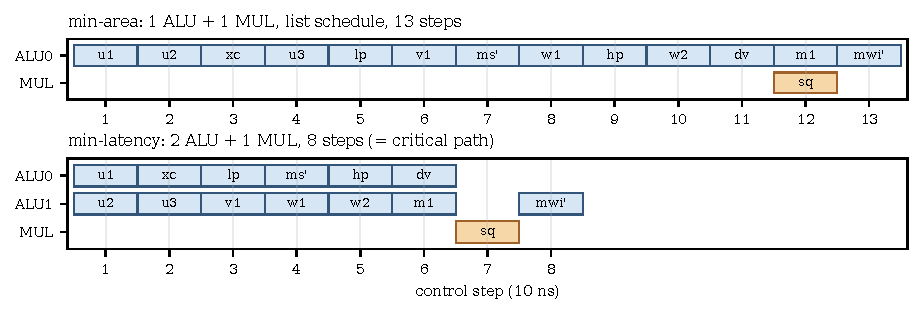
\includegraphics[width=\linewidth]{schedule.pdf}}{\fbox{schedule.pdf}}
\end{minipage}\hfill
\begin{minipage}[c]{0.32\linewidth}\centering
\IfFileExists{compat.pdf}{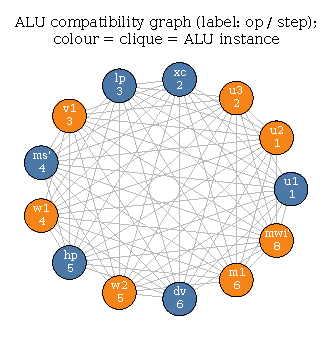
\includegraphics[width=\linewidth]{compat.pdf}}{\fbox{compat.pdf}}
\end{minipage}
\caption{Left: list schedules for 1\,ALU+1\,MUL (13 steps) and 2\,ALU+1\,MUL (8 steps).
Right: ALU compatibility graph of the 8-step schedule, coloured by clique (= ALU instance).}\label{fig:sched}
\end{figure}

\subsection{Allocation and Binding}
\textbf{Registers.} Left-edge allocation on the value lifetimes needs 3 temporaries for the 13-step
schedule and 2 for the 8-step one; values that end a step in an architectural register
($lp\rightarrow lp_1$, $ms'$, $hp$, $dv$, $mwi'$) need none. \textbf{Units.} In the compatibility
graph two ALU operations are compatible if they run in different steps (72 edges for the 8-step
schedule). Clique partitioning gives two units, ALU0 = $\{xc,u_1,lp,ms',hp,dv\}$ (32 bit) and
ALU1 = $\{u_2,u_3,v_1,w_1,w_2,m_1,mwi'\}$ (40 bit, both MWI operations kept together).

\subsection{FSMD and Design Points}
Each control step became one controller state driving the operand-mux selects and register enables
of the bound datapath. We hand-wrote both FSMDs in RTL (\texttt{qrs\_fsmd\_area.v},
\texttt{qrs\_fsmd\_lat.v}); both are bit-exact against the golden model on 20{,}000 samples of record
100 (0 mismatches in \texttt{hp}, \texttt{dv}, \texttt{mwi}). Table~\ref{tab:designpoints} gives
the out-of-context post-route results, with the Vitis-HLS core used on the board as a reference.

\begin{table}[!tbp]\centering\footnotesize\setlength{\tabcolsep}{3.5pt}
\caption{Design points on the FPGA (xc7z010, OOC place and route, 10\,ns target).}\label{tab:designpoints}
\begin{tabular}{@{}lcccccc@{}}
\toprule
Design point & LUT (logic+RAM) & FF & DSP & F$_\text{max}$ (MHz) & Latency (cycles) & Latency (ns)\\
\midrule
Min-latency, 2 ALU + 1 MUL (hand) & 643 (467+176) & 290 & 3 & 110.4 & 8 & 80\\
Min-area, 1 ALU + 1 MUL (hand)    & 670 (494+176) & 345 & 3 & 107.9 & 13 & 130\\
Vitis HLS \texttt{qrs\_stream} (board) & 571 (409+162) & 563 & 3 & 130.1 & 7 (II 8) & 70\\
\bottomrule
\end{tabular}
\end{table}

The ``min-area'' schedule is \emph{not} the smallest circuit: sharing one 40-bit ALU across 13
operations needs two 13-input operand multiplexers, which on a LUT fabric cost more than a second
adder (a 32-bit adder and a 4:1$\times$32 mux both take 32 LUTs). The 2-ALU design is smaller (27
LUTs, 55 FFs) and 5 cycles faster, so on an FPGA the binding cost must include interconnect. All
points use 3 DSP48E1 (the squarer is wider than one $25\times18$ DSP) and need $\le14$ of the
$\approx$69{,}000 cycles per sample.

%% =====================================================================
\section{Logic and FSM Optimisation}
\label{sec:logic}
\subsection{State Minimisation}
We wrote the DDD controller's STG from the specification with one state per timing period
(Fig.~\ref{fig:stg}): VRF (VRP and PVARP running), PVA (A blanked), VRO (V blanked) and ALR (alert)
in the V--A interval; AVD (AV delay) and URW (waiting for URI) in the A--V interval. Its inputs are
$a, v$ and the timer flags $r, b, e, m, u$; impossible flag combinations are don't-cares (288 of 768
entries). The implication chart gives 7 compatible and 8 incompatible pairs and no implied pairs; the
maximal compatibles $\{\mathrm{VRF,PVA,VRO,ALR}\}$, $\{\mathrm{AVD,URW}\}$ form a closed cover, so
the machine \textbf{minimises from 6 to 2 states}. The course kit agrees: its partition step gives
the same classes and \textbf{STAMINA} reports ``6 $\rightarrow$ 2 states, 1 flip-flop''. This is
exactly the phase bit of \texttt{ddd\_pacemaker.v}, because the timer comparators already carry the
blanking information; a product machine and an exhaustive walk of the real timers (249{,}822 states,
five parameter sets) found 0 mismatches. The 8-phase \texttt{qrs\_decision} controller is already
minimal.

\begin{figure}[!tbp]\centering
\begin{minipage}[c]{0.68\linewidth}\centering
\IfFileExists{stg.pdf}{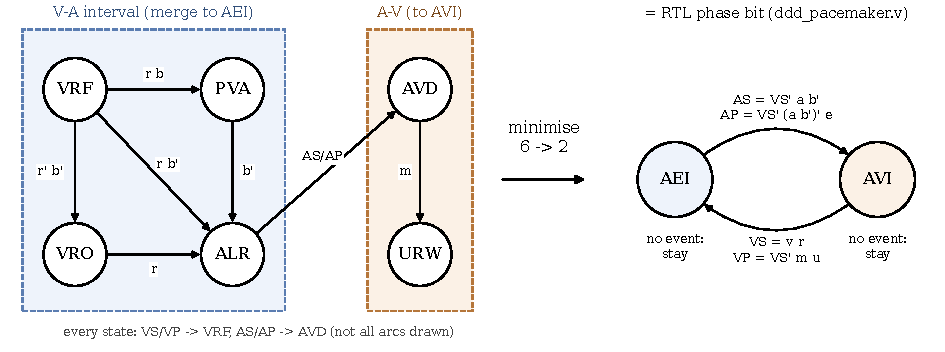
\includegraphics[width=\linewidth]{stg.pdf}}{\fbox{stg.pdf}}
\end{minipage}\hfill
\begin{minipage}[c]{0.27\linewidth}\centering
\IfFileExists{implication.pdf}{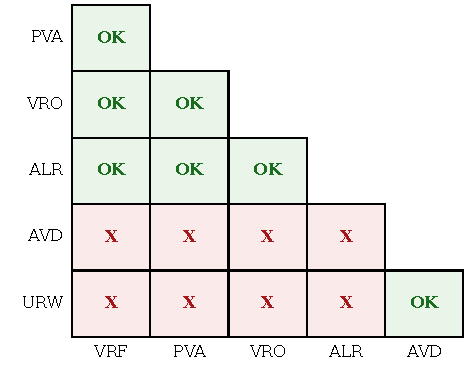
\includegraphics[width=\linewidth]{implication.pdf}}{\fbox{implication.pdf}}
\end{minipage}
\caption{Left: specification STG of the DDD controller, minimised from 6 to 2 states (= the RTL
phase bit). Right: implication chart (OK = compatible, X = outputs differ).}\label{fig:stg}
\end{figure}

\subsection{State Encoding}
The 8-phase sequencer of \texttt{qrs\_decision} (IDLE, TRACK, CLASS, REG, AVG, LIM, SB, END) was
encoded seven ways (Table~\ref{tab:encoding}). The two-level costs come from the course kit
(\texttt{vl401.py encode}, ESPRESSO, with NOVA and JEDI from SIS); our own exact search over all
5{,}040 three-bit codes with IDLE = 000 found that only 6 codes reach the minimum of 42 per-output
literals, and the ``custom'' row is one of them. The FPGA numbers are for the controller alone,
placed and routed with a 2.5\,ns target, and Vivado's synthesis log confirmed each re-encoding.

\begin{table}[!tbp]\centering\footnotesize\setlength{\tabcolsep}{4pt}
\caption{State encodings of the 8-phase controller: kit cost (two-level / multilevel literals) and
xc7z010 implementation.}\label{tab:encoding}
\begin{tabular}{@{}lcccccc@{}}
\toprule
Encoding & State bits & Products / per-output lits & SIS multilevel lits & LUT & FF & F$_\text{max}$ (MHz)\\
\midrule
Binary (as written / sequential) & 3 & 10 / 46 & 38 & 11 & 3 & 595.9\\
Gray & 3 & 10 / 51 & 39 & 11 & 3 & 572.7\\
Johnson & 4 & -- & -- & 14 & 4 & 478.2\\
One-hot & 8 & 11 / 36 & 21 & 7 & 8 & 356.3\\
NOVA (kit) & 3 & 10 / 68 & 46 & -- & -- & --\\
JEDI (kit) & 3 & 11 / 48 & 36 & -- & -- & --\\
Custom (exact minimum) & 3 & 10 / 42 & 33 & 11 & 3 & 541.4\\
\bottomrule
\end{tabular}
\end{table}

The custom code's literal savings (42 vs 46) vanish on the FPGA: every next-state bit fits one LUT6,
so all 3-bit codes cost 11 LUTs; one-hot saves LUTs but adds five FFs and was slowest (Vivado gave it a
shared clock-enable). In the whole \texttt{qrs\_decision} module all encodings give 3{,}619--3{,}641
LUTs and 96--102\,MHz, since the 40-bit datapath, not the controller, is critical. The custom-coded
detector stayed bit-exact (814/814 detections).

\subsection{Two-Level Minimisation}
The event-priority block maps the phase $p$, the senses $a, v$ and the timer flags
$r, m, u, e, b$ (8 inputs) to VS, VP, AS, AP with priority VS $>$ VP $>$ AS $>$ AP. The kit's
ESPRESSO reduced the 148 ON rows to \textbf{9 products / 34 literals}, and \texttt{-Dexact} gave the
same cost. Our own Quine--McCluskey implementation finds 9 prime implicants, all of them essential,
so the covering table empties in one step (no cyclic core, so neither dominance nor branch-and-bound
is needed), and the cover is identical cube for cube to ESPRESSO's:
$\mathrm{VS}=vr$, $\mathrm{VP}=pv'mu+pr'mu$, $\mathrm{AS}=p'av'b'+p'ar'b'$,
$\mathrm{AP}=p'a'v'e+p'a'r'e+p'v'eb+p'r'eb$. The RTL \texttt{event\_priority.v} is written from these
nine products (256/256 input combinations checked in simulation).

\subsection{Multilevel Optimisation}
Kernel extraction finds the common kernel $v'+r'$ with co-kernels $pmu$ (VP), $p'ab'$ (AS) and
$p'a'e$, $p'eb$ (AP), plus $a'+b$ in AP. Extracting them gives 18 literals, the same as the
factored form. SIS \texttt{script.rugged} goes further to \textbf{14 literals}:
$\mathrm{VP}=\mathrm{VS}'mpu$, $\mathrm{AS}=\mathrm{VS}'ab'p'$, $\mathrm{AP}=\mathrm{VS}'\,\mathrm{AS}'ep'$.
Boolean resubstitution notices that $v'+r'=\mathrm{VS}'$ and so recovers the priority chain, which
algebraic kernels cannot. Yosys+ABC on the RTL gives 16 literals with \texttt{fx} (the same chain
structure) and 18 with \texttt{resyn2}; \texttt{abc -lut 6} maps the block to \textbf{4 LUTs},
equal to Vivado (one LUT6 per output is the floor, since each output depends on at most 8 inputs).

%% =====================================================================
\section{RTL Design and SoC Integration}
\label{sec:rtl}
\subsection{Module Hierarchy}
The SoC is an IP-Integrator block design (Fig.~\ref{fig:bd}, appendix) of the blocks in
Fig.~\ref{fig:block}: NEORV32~\cite{neorv32} (RV32I, Zicntr, 16\,KB IMEM with our firmware, 8\,KB
DMEM), SmartConnect, our AXI4-Lite-to-3$\times$APB3 bridge and APB slaves, the HLS IP
\texttt{qrs\_stream} with RTL \texttt{qrs\_decision}, the heart loop (\texttt{heart\_model},
\texttt{ecg\_source}), the display (\texttt{ecg\_display}, \texttt{hdmi\_tx} with OSERDESE2) and
board I/O. Decisions: one 25\,MHz clock domain (125\,MHz only in the HDMI serialiser), synchronous
active-low reset, one-cycle \emph{valid} strobes per sample and tick, an \texttt{ap\_ctrl\_hs}
handshake to the HLS core, and debounced inputs. Verilator \texttt{--lint-only -Wall}: 0 errors; the
remaining warnings are reviewed waivers (blocking temporaries mirroring the golden model, intended
zero-extension, unused APB bits).

\subsection{Bus Integration, Interrupt and DMA}
The CPU's AXI4 master reaches our bridge through the SmartConnect; the bridge decodes the 64\,KB
window at 0x9000\_0000 into three APB windows (Table~\ref{tab:regmap}) with no wait states. The
pacemaker latches its upper-rate flag and drives the CPU's machine external interrupt. The handler
(Listing~\ref{lst:driver}) lengthens PVARP by 50\,ms (max 400) when the PMT-guard switch is on and
clears the flag (write-1-to-clear); with the guard off it masks the interrupt and LED3 stays on. No
DMA is needed: one 11-bit sample arrives every 2.8\,ms and flows from BRAM straight into the hardware
detector, so the CPU only touches control registers.

\begin{lstlisting}[language=C,caption={Driver excerpt: range check before any APB write, and the PMT handler.},label={lst:driver}]
ddd_status_t ddd_set_params(uint32_t lri, uint32_t avi, uint32_t uri, uint32_t pvarp, uint32_t vrp) {
    if (lri < 400u || lri > 2000u)    return DDD_ERR_LRI;      /* rejected: nothing written */
    if (avi < 30u  || avi > 350u)     return DDD_ERR_AVI;
    if (uri < 300u || uri > lri)      return DDD_ERR_URI;      /* + PVARP, VRP, order checks */
    DDD_LRI = lri; DDD_AVI = avi; DDD_URI = uri; DDD_PVARP = pvarp; DDD_VRP = vrp;
    return DDD_OK;
}
void ddd_isr(void) {                                  /* machine external interrupt */
    if (DDD_STATUS & DDD_STAT_ARRHYTHMIA) {
        if (DDD_PVARP < 400u) DDD_PVARP += 50u;       /* stop tracking retrograde P */
        DDD_CONTROL = DDD_CTRL_ENABLE | DDD_CTRL_CLR_ARRH;   /* W1C */
        DDD_CONTROL = DDD_CTRL_ENABLE;
    }
}
\end{lstlisting}

\subsection{Hardware/Software Comparison}
A C port of the same per-sample detector ran on the board's NEORV32 configuration (RV32I, no M
extension, \texttt{-Os}) in RTL simulation of the core, timed with \texttt{mcycle} over 2{,}048
samples of record 100; its outputs and detections equal the golden model. The hardware path was
measured in simulation over 100{,}000 samples (341 detections, bit-exact).

\begin{table}[!tbp]\centering\footnotesize\setlength{\tabcolsep}{4pt}
\caption{Cycles per ECG sample on the same 25\,MHz system.}\label{tab:hwsw}
\begin{tabular}{@{}lccc@{}}
\toprule
Path & SW (RV32I) mean [range] & HW mean & Speed-up\\
\midrule
Filter chain (software multiply, libgcc) & 898.8 [526--1{,}195] & 10 & 89.9$\times$\\
Adaptive-threshold decision & 484.6 [368--2{,}531] & 8.0 & 60.6$\times$\\
\textbf{Total} & \textbf{1{,}383.4} (55.3\,\textmu s) & \textbf{18.0} (0.72\,\textmu s) & \textbf{76.9$\times$} (206$\times$ worst case)\\
\bottomrule
\end{tabular}
\end{table}

Without the M extension the squarer is a shift-add loop, so software time depends on the data. If
the CPU read one result per sample (7 bus cycles), 99.5\,\% of the loop is accelerated and Amdahl's law
gives 55.6$\times$ overall (at most 199$\times$). Software alone would still keep up at 360\,Hz (2\,\%
CPU load); the hardware's value is a fixed 18-cycle latency and a free CPU.

%% =====================================================================
\section{Simulation-Based Verification}
\label{sec:sim}
Every testbench is self-checking: it replays golden-model stimulus and compares every output on
every tick or sample. Directed tests cover the three pacing regimes, six closed-loop heart scenarios
including PMT, all 256 event-priority inputs, two MIT-BIH records through the detector, the bridge,
and the whole SoC running the real firmware. The \textbf{constrained-random} test drives 60 random legal parameter
sets (biased to range ends) with random atrial and ventricular activity for 5{,}000 ticks each,
checks AS/VS/AP/VP and the upper-rate flag every tick, reads back every register and clears 535
latched interrupts by W1C. Nineteen SVA assertions (Listing~\ref{lst:sva}; all in
Table~\ref{tab:svalist}, appendix) are \texttt{bind}-ed to the unmodified RTL.

\begin{lstlisting}[language=Verilog,caption={Two of the 19 SVA assertions (bound to \texttt{ddd\_pacemaker}).},label={lst:sva}]
A07_no_vp_before_uri: assert property (disable iff (!rst_n) (step && tv_n < uri) |=> !vp);
A15_v_within_lri:     assert property (disable iff (!rst_n) since_v <= lri + 1'b1); // bounded liveness
\end{lstlisting}

\begin{table}[!tbp]\centering\footnotesize
\caption{Verification summary (xsim, Vivado 2025.2).}\label{tab:simsummary}
\begin{tabularx}{\linewidth}{@{}Xl@{}}
\toprule
Item & Result\\
\midrule
Directed bit-exact testbenches passed & 9/9 (18{,}000 + 72{,}000 ticks, 256 vectors, 340k samples, SoC)\\
Constrained-random ticks compared & 300{,}000 (60 parameter sets): 0 mismatches after 2 fixes\\
Assertions & 19 SVA + 3 covers, 0 failures; functional bins 20/20 hit\\
Code coverage \texttt{ddd\_pacemaker} / \texttt{\_apb} & statement, branch, condition 100\,\% / 100\,\%\\
Toggle coverage & 70.8\,\% / 5.9\,\% (only bits that cannot toggle are missed)\\
Bugs found by simulation & 5 in the design, 1 in a testbench (Table~\ref{tab:bugs})\\
\bottomrule
\end{tabularx}
\end{table}

Toggle coverage misses only bits that cannot move (timer bits above 2000\,ms, unused APB data bits).
Functional bins include A senses ignored in PVARP (1{,}295), V senses ignored in VRP (1{,}954), VP held
by URI (16{,}484 ticks), simultaneous A and V (627) and every parameter at both range ends.

\begin{table}[!tbp]\centering\footnotesize
\caption{Bugs found by simulation.}\label{tab:bugs}
\begin{tabularx}{\linewidth}{@{}lXX@{}}
\toprule
Found by & Symptom & Root cause and fix\\
\midrule
Random test & first cycle late after enabling with LRI $>1000$\,ms (96 mismatches) &
$t_v$ took the \emph{reset} LRI, not the programmed one; hold the start state while disabled\\
Random test & false PMT interrupt when URI = LRI (8 mismatches) & $t_v$ saturated at LRI, so
``later than LRI'' looked like ``at URI''; saturate at LRI+1\\
Golden replay & first pacing tick one off & reset value of $t_v$ differed from the model\\
Golden replay & NPKI wrong on negative differences & signed/unsigned concatenation in \texttt{qrs\_decision}\\
HLS C-sim & first outputs of a record differed & delay lines not zero-initialised like the model\\
Baseline TB & every detection one sample late & testbench drove inputs with blocking assignments on the sampling edge\\
\bottomrule
\end{tabularx}
\end{table}

Assertion A10 ($t_v\le$ LRI) also fired once, just after software wrote a \emph{smaller} LRI: the
timer is clamped only at the next tick, before use, so the property was restated ``after every tick''.

%% =====================================================================
\section{Formal Verification}
\label{sec:formal}
All models use the current RTL (with the two fixes of Section~\ref{sec:sim}) and abstract time to
ticks: AVI\,=\,2, VRP\,=\,3, PVARP\,=\,4, URI\,=\,5, LRI\,=\,10, AEI\,=\,8.

\subsection{Kripke Structure and CTL Labelling}
Figure~\ref{fig:kripke} is the 16-state Kripke structure of the controller with PVARP blanking
removed (bug~1), in closed loop with a heart that has AV block and a retrograde P wave 3 ticks after
each V beat; \textit{upper} labels a V beat at URI (s11), \textit{slow} the other V beats (s3). By
hand, the least fixpoint for $\varphi_1=\Eu[\neg\mathit{upper}\,\mathbf{U}\,\mathrm{AS}]$ grows
$Z_0=\{s7\}$ by predecessors outside \textit{upper} ($s5, s4, s3, \{s2,s15\},\ldots$) to all states
except $s9, s11$; the greatest fixpoint for $\varphi_2=\EG\neg\mathit{slow}$ shrinks ``all but $s3$''
to $\{s4,s5,s7,s9,s11\}$, exactly the PMT loop. NuSMV labels the same states, and since
$\EF\EG\neg\mathit{slow}$ holds at reset, P11 below must fail under bug~1.

\figfloat{kripke.pdf}{0.72\linewidth}{Kripke structure of the controller with the PVARP bug and a
retrograde-conducting heart. Red: $\EG\neg\mathit{slow}$ holds (the PMT loop); $\Eu[\neg
\mathit{upper}\,\mathbf{U}\,\mathrm{AS}]$ holds everywhere except s9 and s11.}{fig:kripke}

\subsection{Model Checking with NuSMV}
The NuSMV model (Appendix~\ref{app:nusmv}) mirrors \texttt{ddd\_pacemaker.v} register by register:
\texttt{phase}, $t_v$ (saturating at LRI+1) and $t_{av}$, with the per-tick priority VS $>$ VP $>$ AS
$>$ AP written as DEFINEs. The 1\,ms \texttt{tick} and the heart events $a$, $v$ are free inputs, so
the proofs cover every possible heart (168 reachable states, diameter 11, $\approx$50\,ms per run).
Table~\ref{tab:ctl} lists the 12 properties.

\begin{table}[!tbp]\centering\footnotesize\setlength{\tabcolsep}{3.5pt}
\caption{CTL properties checked with NuSMV 2.7.1 (over-approximating heart; P11 uses the AV-block +
retrograde heart; P0 checks that bounding $t_{av}$ loses no behaviour).}\label{tab:ctl}
\begin{tabularx}{\linewidth}{@{}clXcc@{}}
\toprule
\# & Type & CTL formula & No fairness & \texttt{FAIRNESS tick}\\
\midrule
P0 & Abstraction & $\AG\, t_{av}\le 4$ & true & true\\
P1 & Safety & $\AG\,\neg(\mathrm{AP}\wedge\mathrm{VP})$ & true & true\\
P2 & Safety (upper rate) & $\AG(\mathrm{VP}\rightarrow t_v\ge\mathrm{URI})$ & true & true\\
P3 & Safety (PVARP) & $\AG(\mathrm{AS}\rightarrow t_v\ge\mathrm{PVARP})$ & true & true\\
P4 & Safety (VRP) & $\AG(\mathrm{VS}\rightarrow t_v\ge\mathrm{VRP})$ & true & true\\
P5 & Safety (AV delay) & $\AG(\mathrm{VP}\rightarrow t_{av}\ge\mathrm{AVI})$ & true & true\\
P6 & Safety (escape) & $\AG(\mathrm{AP}\rightarrow t_v\ge\mathrm{AEI})$ & true & true\\
P7 & Reachability & $\EF\mathrm{AP}\wedge\EF\mathrm{VP}\wedge\EF\mathrm{AS}\wedge\EF\mathrm{VS}$ & true & true\\
P8 & Non-blocking & $\AG\,\EF(\mathit{phase}=\mathrm{AEI})$ & true & true\\
P9 & Liveness & $\AG\,\AF(\mathrm{VS}\vee\mathrm{VP})$ & \textbf{false} & true\\
P10 & Until & $\AG((\mathrm{AS}\vee\mathrm{AP})\rightarrow\AX\,\Au[\neg(\mathrm{AS}\vee\mathrm{AP})\,\mathbf{U}\,(\mathrm{VS}\vee\mathrm{VP})])$ & \textbf{false} & true\\
P11 & No PMT & $\AG\,\AF\,\mathit{slow\_vbeat}$ & -- & true; \textbf{false} with bug 1\\
\bottomrule
\end{tabularx}
\end{table}

P9 and P10 fail without fairness because \texttt{tick} is a free input: NuSMV returns a lasso in
which the 1\,ms time base simply stops (at reset, or in the AVI phase after an AP).
\texttt{FAIRNESS tick} models a working timer, and both then hold. P0 shows that bounding $t_{av}$
cuts no reachable behaviour.

\subsection{Bug Injection and Counterexamples}
\textbf{Bug~1} (PVARP blanking removed) makes P3 fail and, with the retrograde heart, P11 fail with
an 11-state lasso: AP, slow VP, AS of the retrograde P inside PVARP, VP at URI, repeat (the PMT).
\textbf{Bug~2} (VRP blanking removed) makes P4 fail with a 3-state trace. Replaying each
counterexample in xsim on a one-line mutant of the RTL, one NuSMV state per clock, gave 0 register
and output mismatches (34 cycles for the unrolled lasso), while the correct RTL diverges exactly where
the bug acts. In closed loop the bug-1 RTL paced 7 of 8 V beats at the upper rate and the correct RTL
none (Fig.~\ref{fig:replay}, appendix).

\subsection{BDD Analysis}
With the \texttt{dd} package we built one shared ROBDD for the four event-priority outputs
(Table~\ref{tab:bdd}). The variable order changes the size by more than 2$\times$; dynamic
sifting improves the natural order by 22\,\% but stays above the exhaustive optimum over all
$8!=40{,}320$ orders, which only 0.6\,\% of the orders reach. In one manager, the truth table, the
ESPRESSO SOP, the kit's factored, kernel and \texttt{script.rugged} forms, the RTL equations and the
Yosys/ABC netlist all map to the \emph{same} root nodes, which proves them equivalent. Symbolic
reachability by BDD image computation gives the same reachable-state counts as NuSMV for all five
models (168, 26, 16, 240 and 168 states).


\subsection{Formal Verification of the RTL (SymbiYosys)}
A harness with free inputs assumes a reset, a legal parameter set as in the driver's range check,
and parameters that change only while the controller is disabled. Eight assertions are added to a
copy of \texttt{ddd\_pacemaker.v} through one \texttt{\textasciigrave include} under \texttt{\textasciigrave ifdef FORMAL}: A1 no
AP with VP; A2--A4 no VP before URI, no AS inside PVARP, no VS inside VRP (measured by an
independent tick counter); A5 a V event at least every LRI; A6 $t_v\le$ LRI+1; A7 phase/timer
consistency; A8 the first cycle after enable uses the programmed LRI. k-induction needed five
proven strengthening invariants (e.g.\ the counter equals $t_v$; a stored AVI state never has both
AVI and URI elapsed); without them it failed even at $k=30$ on unreachable states.

\begin{table}[!tbp]\centering\scriptsize\setlength{\tabcolsep}{2.5pt}
\begin{minipage}[t]{0.40\linewidth}\centering
\caption{Shared ROBDD nodes, event-priority block (classical incl.\ terminals; \texttt{dd} with complement edges).}\label{tab:bdd}
\begin{tabular}{@{}lcc@{}}
\toprule
Variable ordering & Classical & \texttt{dd}\\
\midrule
Natural $p\ldots b$ & 23 & 21\\
Reversed $b\ldots p$ & 22 & 20\\
Timers first & 26 & 22\\
Worst of 8! orders & 32 & 29\\
Dynamic sifting & 18 & 15\\
Exhaustive optimum & \textbf{15} & \textbf{12}\\
\bottomrule
\end{tabular}
\end{minipage}\hfill
\begin{minipage}[t]{0.58\linewidth}\centering
\caption{SymbiYosys (smtbmc with Yices/Bitwuzla).}\label{tab:sby}
\begin{tabular}{@{}llcc@{}}
\toprule
Task & Design & Result & Depth / $k$\\
\midrule
BMC & fixed RTL, $W=8$ & pass & 40 steps\\
k-induction & fixed RTL, $W=8$ & \textbf{proved} & $k=3$\\
k-induction & $W=16$, firmware ranges & \textbf{proved} & 12\\
BMC & RTL before start-up fix & \textbf{A8 fails} & step 3\\
BMC & bug-1 / bug-2 mutant & \textbf{A3 / A4 fail} & step 4\\
\bottomrule
\end{tabular}
\end{minipage}
\end{table}

So the safety properties hold for \emph{all} legal 16-bit parameter sets, not only the abstract
ones, and the start-up bug that random simulation found is also caught independently by A8.

%% =====================================================================
\section{Incorporating the Research Paper}
\label{sec:paper}
Our first demo detector was a fixed threshold on the raw ECG (B0). Following Pan and
Tompkins~\cite{pan} we replaced it with their pipeline: the filter chain of Section~\ref{sec:hls} and
an RTL decision stage that keeps signal and noise peak estimates (SPKI, NPKI, weight 1/8), sets
$\mathrm{THR1}=\mathrm{NPKI}+(\mathrm{SPKI}-\mathrm{NPKI})/4$ and $\mathrm{THR2}=\mathrm{THR1}/2$
(halved for an irregular rhythm), rejects T waves whose slope is below half that of the last QRS
within 360\,ms, applies a 200\,ms refractory period, and searches back with THR2 when no beat is found
within 166\,\% of the mean R--R interval. Every constant is a shift-add (e.g.\
$0.92a=a-a/16-a/64$), so no multiplier is needed. To separate the two parts of the technique we also
built B1: the same filters with a fixed MWI threshold. B0 and B1 were tuned on record 100 only and then
frozen, as a hardware constant would be. All three detectors are bit-exact RTL against Python and were
placed and routed on the same device with the same 10\,ns constraint (Table~\ref{tab:paper}).

\begin{table}[!tbp]\centering\footnotesize\setlength{\tabcolsep}{3.5pt}
\caption{Baseline vs.\ paper-enhanced detector (5 records, 11{,}873 beats, $\pm150$\,ms; xc7z010 OOC, 10\,ns).}\label{tab:paper}
\begin{tabular}{@{}lcccc@{}}
\toprule
Metric & B0: fixed threshold & B1: PT filters + fixed thr. & E: full Pan--Tompkins & B0$\rightarrow$E\\
\midrule
Gross \Se{} (\%) & 98.56 & 99.21 & \textbf{99.55} & $+0.99$\\
Gross \Pp{} (\%) & 88.36 & 98.40 & \textbf{99.92} & $+11.56$\\
FP / FN & 1{,}541 / 171 & 192 / 94 & \textbf{9 / 53} & FP $-99.4\,\%$\\
LUT / FF & 16 / 73 & 510 / 619 & 2{,}850 / 2{,}385 & $+2{,}834$ LUT\\
DSP / BRAM & 0 / 0 & 3 / 0 & 3 / 0 & +3 DSP\\
F$_\text{max}$ (MHz) & 256 & 136 & 96 & (board: 25)\\
Decision delay after R peak & $-15$\,ms & $+14$\,ms & $+217$\,ms & \\
\bottomrule
\end{tabular}
\end{table}


The filters alone (B1) remove most of B0's false detections, and the adaptive thresholds remove almost
all of the rest (192 $\rightarrow$ 9) while recovering missed beats (94 $\rightarrow$ 53). B0's
perfect score on record 100 is overfitting to its training record: the same constant gives
\Pp{} = 64.2\,\% on record 106 (Fig.~\ref{fig:paper106}, appendix). The paper's headline ``99.3\,\%'' is not a
sensitivity but $1-(\mathrm{FP}+\mathrm{FN})/\text{beats}$ over the 24\,h database~\cite{pan}; on that
measure we obtain 99.48\,\%. On the paper's own per-record table for our five records
(Table~\ref{tab:lit}) our \Pp{} matches theirs (99.92 vs 99.88\,\%) but our \Se{} is lower (99.55 vs
99.84\,\%; 53 vs 19 misses). 30 of our 53 misses are PVCs (2.0\,\% of 1{,}516 PVCs vs 0.2\,\% of normal
beats; 19 of 20 on record 106): wide, low-slope PVCs are what our fixed-point slope test handles worst,
since we kept the paper's rules unchanged at 360\,Hz and used a strict $\pm150$\,ms window (the paper
states none). The technique costs 2{,}834 LUTs and a 217\,ms decision delay, still well before the next
beat.

\begin{table}[!tbp]\centering\footnotesize\setlength{\tabcolsep}{3pt}
\caption{Research comparison. Accuracy on \emph{our five records} is derived from each paper's
per-record table; resources are not directly comparable across FPGA families.}\label{tab:lit}
\begin{tabular}{@{}lllcc@{}}
\toprule
Work & Platform & Resources & \Se{} / \Pp{} (5 rec.) & \Se{} / \Pp{} (all)\\
\midrule
Pan \& Tompkins~\cite{pan} & Z80 software, 200\,Hz & -- & 99.84 / 99.88 & 99.76 / 99.56\\
Cvikl et al.~\cite{cvikl} & Virtex-II FPGA, 250\,Hz & $\approx$17\,\% of XC2V3000 & 99.87 / 99.94 & 99.82 / 99.82\\
Chen et al.~\cite{chen} & Cyclone~V FPGA & 22{,}332 ALM, 87 DSP & 99.92 / 99.95$^{\dagger}$ & 99.85 / 99.93$^{\dagger}$\\
Ieong et al.~\cite{ieong} & 0.35\,\textmu m ASIC & 0.83\,\textmu W & -- & 99.31 / 99.70\\
\textbf{This work} & xc7z010, 360\,Hz integer & 2{,}850 LUT, 3 DSP, 0 BRAM & \textbf{99.55 / 99.92} & --\\
\bottomrule
\multicolumn{5}{@{}l}{\footnotesize $^{\dagger}$300\,ms matching window; ours is $\pm150$\,ms. Tolerances of~\cite{pan,cvikl} are not stated.}
\end{tabular}
\end{table}

%% =====================================================================
\section{FPGA Implementation and Demonstration}
\label{sec:fpga}
\begin{table}[!tbp]\centering\footnotesize
\caption{Post-implementation results on the Zybo Z7-10 (xc7z010clg400-1).}\label{tab:fpga}
\begin{tabular}{@{}lcc@{}}
\toprule
Item & SoC (\texttt{p17\_soc}) & SoC + ILA/VIO, rebuilt with fixes\\
\midrule
Target clock (MHz) & 25 & 25\\
WNS / WHS (ns) & $+23.598$ / $+0.040$ & $+23.737$ / $+0.020$\\
LUT / FF & 6{,}772 (38.5\,\%) / 5{,}360 (15.2\,\%) & 9{,}939 (56.5\,\%) / 10{,}774\\
DSP / BRAM36 & 3 / 19.5 & 3 / 41.5\\
Estimated power (W) & 0.355 (0.258 dynamic + 0.097 static) & 0.366\\
\bottomrule
\end{tabular}
\end{table}

Power is Vivado's post-route vectorless estimate (confidence ``low''); the Zybo has no supply-current
sensor. Clocking (MMCM, 0.106\,W) and the HDMI TMDS outputs (0.136\,W) dominate; detector, pacemaker
and CPU together use about 0.02\,W. The on-chip XADC, read over JTAG with the design running, showed
38.0\,$^\circ$C and VCCINT 0.998\,V. Per-block resources are in Table~\ref{tab:perblock}.

\textbf{Demonstration.} LD0/LD1 flash on each atrial/ventricular pace, LD2 on each detected QRS and
LD3 on the arrhythmia interrupt; BTN1 steps through six scenarios, BTN2 requests a new lower rate
(accepted) and BTN3 LRI = 300\,ms (rejected by the range check); SW0 enables pacing, SW1 the PMT guard.
The ECG with beat markers is drawn at $640\times480$ on the HDMI port (the Zybo Z7-10 has no VGA
connector; the same timing is sent as DVI). With no monitor in the lab, an ILA storing one entry per
360\,Hz sample captured the running design and the ECG was rebuilt in Python (Fig.~\ref{fig:ila}). All seven 22.8\,s captures were contiguous and match simulation, and repeating them with the
rebuilt bitstream gave identical counts (Table~\ref{tab:board}, appendix), e.g.\
28/28 beats detected on record 100 and a 120\,bpm PMT returned to 60\,bpm by the RV32 handler.

\figfloat{fig_ila_board.pdf}{0.84\linewidth}{ILA captures from the running Zybo: record 100 with on-chip
detections; the PMT scenario with the guard off (VP at the upper rate) and on (RV32 handler, back to
60\,bpm).}{fig:ila}

%% =====================================================================
\section{Discussion and Limitations}
\label{sec:discussion}
\textbf{What worked.} Writing every block first as a bit-exact integer model made each RTL step
checkable sample by sample, and the same models drove the formal abstractions and the paper
comparison. Constrained-random stimulus found two corner-case bugs that 90{,}000 directed ticks missed,
because the directed tests used only default parameters. Hand HLS showed that the recurrence
transformation, not resource sharing, makes the filter small, and that on an FPGA the fewest
functional units is not the smallest circuit.

\textbf{Limitations.} (i) The HDMI display was never seen on a monitor (none in the lab); the ECG and
markers were shown through the ILA and the screen was checked in simulation. (ii) Power is a
vectorless estimate. (iii) The detector was scored on 5 of 48 records and one lead; in AV-sequential
pacing its fiducial lands on the atrial pacing artefact (still one detection per beat). (iv) The two
controller fixes came after the board measurements; they only affect the first cycle after enabling
with LRI $>1000$\,ms and URI = LRI, which no board scenario uses; all regressions were re-run, and the
rebuilt bitstream (timing met, +11 LUTs) gave identical board captures.
(v) The SymbiYosys proofs cover safety at full width; liveness relies on a fair 1\,ms time base.

\textbf{What we would do differently:} start constrained-random testing and assertions on day one,
and give interconnect a cost in the binding step.

%% =====================================================================
\section{Conclusion and Future Work}
\label{sec:conclusion}
The detector reaches \Se{} 99.55\,\% / \Pp{} 99.92\,\% on five MIT-BIH records with 2{,}850 LUTs, 3 DSPs
and 18 cycles per sample (77$\times$ faster than software on the same core); the paper's adaptive
thresholds remove 99.4\,\% of a fixed threshold's false detections. The DDD controller paces correctly
in all six closed-loop scenarios on the board, its RV32 handler turns a 120\,bpm PMT back into
60\,bpm, and it is proved safe for every legal parameter set. Future work: evaluate all 48 records
with the full EC57 protocol and raise PVC sensitivity (e.g.\ a width-aware T-wave test); add DDD
mode switching and verify it with the same NuSMV/SymbiYosys flow.

%% =====================================================================
\section*{Contribution Statement and Acknowledgements}
\addcontentsline{toc}{section}{Contribution Statement and Acknowledgements}
\label{sec:contrib}
\begin{table}[H]\centering\small
\begin{tabularx}{\linewidth}{@{}lX@{}}
\toprule
Member & Main contributions\\
\midrule
\studentA & Golden models and MIT-BIH evaluation, Pan--Tompkins paper study and baseline
comparison, hand HLS (CDFG, scheduling, binding), logic and FSM optimisation with the course kit.\\
\studentB & RTL of the pacemaker, detector decision stage and SoC, NEORV32 firmware and
block design, Zybo bring-up and ILA demo, simulation and formal verification.\\
\bottomrule
\end{tabularx}
\end{table}
Both members reviewed all parts and can explain them in the viva.

\textbf{Open-source IP and data:} NEORV32 RISC-V processor (BSD-3-Clause)~\cite{neorv32}; AMD/Xilinx
IP (Clocking Wizard, Processor System Reset, AXI SmartConnect, ILA, VIO) and Vitis HLS~\cite{ug1399};
the course's Digital Logic Synthesis Kit (Berkeley SIS/ESPRESSO)~\cite{vl401kit}; NuSMV~2.7.1~\cite{nusmv};
Yosys, SymbiYosys, Verilator and the SMT solvers of the OSS CAD Suite~\cite{yosys}; the Python
\texttt{dd} BDD package; the MIT-BIH Arrhythmia Database from PhysioNet~\cite{moody,goldberger}.

\textbf{AI-tool use:} an AI assistant was used to explain NuSMV syntax errors. An AI coding
assistant (Anthropic Claude, used through Claude Code) helped throughout the project: writing and
debugging RTL, testbenches, Python models and tool scripts.

%% =====================================================================
\begin{thebibliography}{99}\small
\bibitem{pan} J.~Pan and W.~J. Tompkins, ``A real-time {QRS} detection algorithm,'' \emph{IEEE Trans. Biomed. Eng.}, vol. BME-32, no.~3, pp. 230--236, Mar. 1985, doi: 10.1109/TBME.1985.325532.
\bibitem{hamilton} P.~S. Hamilton and W.~J. Tompkins, ``Quantitative investigation of {QRS} detection rules using the {MIT/BIH} arrhythmia database,'' \emph{IEEE Trans. Biomed. Eng.}, vol. BME-33, no.~12, pp. 1157--1165, Dec. 1986, doi: 10.1109/TBME.1986.325695.
\bibitem{elgendi} M.~Elgendi, ``Fast {QRS} detection with an optimized knowledge-based method: Evaluation on 11 standard {ECG} databases,'' \emph{PLoS ONE}, vol.~8, no.~9, Art. no. e73557, Sep. 2013, doi: 10.1371/journal.pone.0073557.
\bibitem{cvikl} M.~Cvikl, F.~Jager, and A.~\v{Z}emva, ``Hardware implementation of a modified delay-coordinate mapping-based {QRS} complex detection algorithm,'' \emph{EURASIP J. Adv. Signal Process.}, vol.~2007, Art. no.~57286, 2007, doi: 10.1155/2007/57286.
\bibitem{chen} A.~Chen, Y.~Zhang, M.~Zhang, W.~Liu, S.~Chang, H.~Wang, J.~He, and Q.~Huang, ``A real time {QRS} detection algorithm based on {ET} and {PD} controlled threshold strategy,'' \emph{Sensors}, vol.~20, no.~14, Art. no.~4003, Jul. 2020, doi: 10.3390/s20144003.
\bibitem{ieong} C.-I. Ieong, P.-I. Mak, C.-P. Lam, C.~Dong, M.-I. Vai, P.-U. Mak, S.-H. Pun, F.~Wan, and R.~P. Martins, ``A 0.83-$\mu$W {QRS} detection processor using quadratic spline wavelet transform for wireless {ECG} acquisition in 0.35-$\mu$m {CMOS},'' \emph{IEEE Trans. Biomed. Circuits Syst.}, vol.~6, no.~6, pp. 586--595, Dec. 2012, doi: 10.1109/TBCAS.2012.2188798.
\bibitem{jiang_tacas} Z.~Jiang, M.~Pajic, S.~Moarref, R.~Alur, and R.~Mangharam, ``Modeling and verification of a dual chamber implantable pacemaker,'' in \emph{Proc. TACAS}, LNCS vol.~7214. Springer, 2012, pp. 188--203, doi: 10.1007/978-3-642-28756-5\_14.
\bibitem{bsc} Boston Scientific, ``{PACEMAKER} system specification,'' Jan. 2007. [Online]. Available: \url{https://sqrl.cas.mcmaster.ca/_SQRLDocuments/PACEMAKER.pdf}
\bibitem{bernstein} A.~D. Bernstein \emph{et al.}, ``The revised {NASPE/BPEG} generic code for antibradycardia, adaptive-rate, and multisite pacing,'' \emph{Pacing Clin. Electrophysiol.}, vol.~25, no.~2, pp. 260--264, Feb. 2002, doi: 10.1046/j.1460-9592.2002.00260.x.
\bibitem{moody} G.~B. Moody and R.~G. Mark, ``The impact of the {MIT-BIH} arrhythmia database,'' \emph{IEEE Eng. Med. Biol. Mag.}, vol.~20, no.~3, pp. 45--50, 2001, doi: 10.1109/51.932724.
\bibitem{goldberger} A.~L. Goldberger \emph{et al.}, ``{PhysioBank}, {PhysioToolkit}, and {PhysioNet}: Components of a new research resource for complex physiologic signals,'' \emph{Circulation}, vol.~101, no.~23, pp. e215--e220, Jun. 2000, doi: 10.1161/01.CIR.101.23.e215.
\bibitem{ec57} \emph{Testing and Reporting Performance Results of Cardiac Rhythm and {ST} Segment Measurement Algorithms}, ANSI/AAMI EC57:2012/(R)2020, AAMI, 2012.
\bibitem{demicheli} G.~De~Micheli, \emph{Synthesis and Optimization of Digital Circuits}. New York, NY, USA: McGraw-Hill, 1994.
\bibitem{paulin} P.~G. Paulin and J.~P. Knight, ``Force-directed scheduling for the behavioral synthesis of {ASICs},'' \emph{IEEE Trans. Comput.-Aided Des. Integr. Circuits Syst.}, vol.~8, no.~6, pp. 661--679, Jun. 1989, doi: 10.1109/43.31522.
\bibitem{kurdahi} F.~J. Kurdahi and A.~C. Parker, ``{REAL}: A program for {REgister ALlocation},'' in \emph{Proc. 24th ACM/IEEE Design Automation Conf.}, 1987, pp. 210--215, doi: 10.1145/37888.37920.
\bibitem{brayton} R.~K. Brayton, G.~D. Hachtel, C.~T. McMullen, and A.~L. Sangiovanni-Vincentelli, \emph{Logic Minimization Algorithms for {VLSI} Synthesis}. Kluwer, 1984, doi: 10.1007/978-1-4613-2821-6.
\bibitem{sis} E.~M. Sentovich \emph{et al.}, ``{SIS}: A system for sequential circuit synthesis,'' Univ. of California, Berkeley, Tech. Rep. UCB/ERL M92/41, May 1992.
\bibitem{clarke} E.~M. Clarke, E.~A. Emerson, and A.~P. Sistla, ``Automatic verification of finite-state concurrent systems using temporal logic specifications,'' \emph{ACM Trans. Program. Lang. Syst.}, vol.~8, no.~2, pp. 244--263, Apr. 1986, doi: 10.1145/5397.5399.
\bibitem{nusmv} A.~Cimatti \emph{et al.}, ``{NuSMV} 2: An {OpenSource} tool for symbolic model checking,'' in \emph{Proc. CAV}, LNCS vol.~2404. Springer, 2002, pp. 359--364, doi: 10.1007/3-540-45657-0\_29.
\bibitem{bryant} R.~E. Bryant, ``Graph-based algorithms for {Boolean} function manipulation,'' \emph{IEEE Trans. Comput.}, vol.~C-35, no.~8, pp. 677--691, Aug. 1986, doi: 10.1109/TC.1986.1676819.
\bibitem{rudell} R.~Rudell, ``Dynamic variable ordering for ordered binary decision diagrams,'' in \emph{Proc. IEEE/ACM ICCAD}, 1993, pp. 42--47, doi: 10.1109/ICCAD.1993.580029.
\bibitem{neorv32} S.~Nolting, ``The {NEORV32} {RISC-V} processor,'' 2020--2026. [Online]. Available: \url{https://github.com/stnolting/neorv32}
\bibitem{yosys} C.~Wolf, ``Yosys Open SYnthesis Suite,'' and YosysHQ, ``SBY (SymbiYosys).'' [Online]. Available: \url{https://yosyshq.net/yosys/}, \url{https://github.com/YosysHQ/sby}
\bibitem{ug1399} AMD, \emph{Vitis High-Level Synthesis User Guide}, UG1399 (v2025.2), 2025.
\bibitem{zybo} Digilent Inc., \emph{Zybo Z7 Board Reference Manual}, rev.~B, Feb. 2018.
\bibitem{vl401kit} B.~Paul, ``Digital Logic Synthesis Kit v1.0 (\texttt{vl401.py} with Berkeley SIS and ESPRESSO),'' A2DSL, IIT Mandi, 2026. [Online]. Available: \url{https://a2dsl.iitmandi.ac.in/resources/1/m/0}
\end{thebibliography}


%% =====================================================================
\appendix
\section{Repository and How to Reproduce}
\label{app:repro}
Layout: \texttt{src/} Python golden models, \texttt{tests/} 48 pytest checks, \texttt{hls/}
Vitis HLS kernels, \texttt{rtl/} RTL, testbenches and firmware, \texttt{vivado/} projects and Tcl,
\texttt{results/} logs and plots, \texttt{report/work/} the experiments of this report
(\texttt{paper}, \texttt{sim}, \texttt{hand\_hls}, \texttt{fsm\_logic}, \texttt{formal},
\texttt{hwsw}, \texttt{lint}, \texttt{refs}). All commands run from the repository root on Windows
(Vivado 2025.2, Python venv, OSS CAD Suite, NuSMV 2.7.1); the course kit runs in Colab.
\begin{lstlisting}[language=bash,numbers=none]
.venv\Scripts\python -m pytest tests -q                       # golden models (48 tests)
.venv\Scripts\python src\evaluate_hw_detector.py              # Se/+P, 5 MIT-BIH records
.venv\Scripts\python report\work\paper\baseline_eval.py       # Sec. 9: B0 / B1 / E
.venv\Scripts\python report\work\sim\run_regression.py        # all xsim testbenches, SVA, coverage
verilator --lint-only -Wall rtl\ddd_pacemaker.v               # lint (each module)
.venv\Scripts\python report\work\hand_hls\hand_hls.py         # Sec. 4 DFGs, schedules, ILP, binding
report\work\hand_hls\impl\run_impl.bat                        # Sec. 4 FSMD design points (Vivado)
python3 vl401.py minimize|encode|twolevel|multilevel <file>   # course kit (Colab), Sec. 5
report\work\fsm_logic\vivado\run_enc.bat ctrl                 # Sec. 5 state encodings (Vivado)
NuSMV -dcx report\work\formal\ddd_oa.smv                      # Sec. 8 CTL properties
sby -f report\work\formal\sby\ddd.sby bmc prove prove16       # Sec. 8 SymbiYosys
hls\run_hls_z7.bat                                            # HLS IP (csim, csynth, export)
vivado -source vivado\create_zybo_bd.tcl                      # SoC block design + bitstream
vivado -mode batch -source vivado\ila_capture_batch.tcl       # board ILA captures
\end{lstlisting}

\section{NuSMV Model (excerpt)}
\label{app:nusmv}
\begin{lstlisting}[language=SMV,caption={Over-approximating DDD model \texttt{ddd\_oa.smv} (excerpt).},label={lst:smv}]
MODULE main
DEFINE
  LRI := 10;  AVI_T := 2;  URI := 5;  PVARP := 4;  VRP := 3;
  AEI := LRI - AVI_T;
VAR
  phase : {PH_AEI, PH_AVI};   -- RTL register 'phase'
  t_v   : 0..11;              -- ticks since last V event (saturates at LRI+1)
  t_av  : 0..10;              -- ticks since the atrial event
  tick  : boolean;            -- 1 ms timebase strobe (free)
  a     : boolean;            -- intrinsic atrial event (free)
  v     : boolean;            -- intrinsic ventricular event (free)
DEFINE
  tv  := min(t_v + 1, LRI + 1);                 -- RTL: (t_v>=lri) ? lri+1 : t_v+1
  tav := (phase = PH_AVI) ? min(t_av + 1, 10) : 0;
  VS := tick & v & tv >= VRP;                    -- priority VS > VP > AS > AP
  VP := tick & !VS & phase = PH_AVI & tav >= AVI_T & tv >= URI;
  AS := tick & !VS & !VP & phase = PH_AEI & a & !(tv < PVARP);
  AP := tick & !VS & !VP & phase = PH_AEI & !AS & tv >= AEI;
  Vbeat := VS | VP;
ASSIGN
  init(phase) := PH_AEI;  init(t_v) := LRI;  init(t_av) := 0;
  next(phase) := case !tick : phase; VS | VP : PH_AEI; AS | AP : PH_AVI; TRUE : phase; esac;
  next(t_v)   := case !tick : t_v;   VS | VP : 0;      TRUE : tv;  esac;
  next(t_av)  := case !tick : t_av;  VS | VP | AS | AP : 0;   TRUE : tav; esac;
FAIRNESS tick
CTLSPEC NAME P1  := AG !(AP & VP);
CTLSPEC NAME P2  := AG (VP -> tv >= URI);
CTLSPEC NAME P3  := AG (AS -> tv >= PVARP);
CTLSPEC NAME P4  := AG (VS -> tv >= VRP);
CTLSPEC NAME P5  := AG (VP -> tav >= AVI_T);
CTLSPEC NAME P6  := AG (AP -> tv >= AEI);
CTLSPEC NAME P7  := EF AP & EF VP & EF AS & EF VS;
CTLSPEC NAME P8  := AG EF phase = PH_AEI;
CTLSPEC NAME P9  := AG AF Vbeat;
CTLSPEC NAME P10 := AG ((AS | AP) -> AX A[ !(AS | AP) U Vbeat ]);
\end{lstlisting}
The full model adds P0, switches for the two injected bugs and the \textit{upper}/\textit{slow\_vbeat}
labels; the PMT model replaces the free $a, v$ with the AV-block + retrograde heart and checks
\texttt{P11 := AG AF slow\_vbeat}.

\section{Additional Material}
\label{app:extra}
\figfile{fig_paper_106.pdf}{0.94\linewidth}{Record 106: the fixed threshold B0 fires on every tall T wave
(8 false detections in 6\,s); the paper's adaptive THR1 tracks the MWI peaks and detects only the QRS
complexes.}{fig:paper106}

\begin{table}[H]\centering\small\setlength{\tabcolsep}{4pt}
\caption{Measured on the board (ILA, 8{,}192 samples = 22.8\,s per scenario); identical with the original and the rebuilt bitstream.}\label{tab:board}
\begin{tabular}{@{}lcccccc@{}}
\toprule
Scenario & HR (bpm) & QRS & AP & VP & AS & VS\\
\midrule
MIT-BIH record 100 replay & 74 & 28 & 0 & 0 & 0 & 28\\
Normal sinus & 75 & 28 & 0 & 0 & 29 & 29\\
Sinus bradycardia & 62 & 24 & 23 & 0 & 0 & 24\\
Complete AV block & 75 & 28 & 0 & 28 & 29 & 0\\
AV block + bradycardia & 60 & 23 & 22 & 23 & 0 & 0\\
Retrograde VA, PMT guard off & 120 & 46 & 0 & 45 & 46 & 0\\
Retrograde VA, PMT guard on (RV32 ISR) & 60 & 23 & 22 & 23 & 0 & 0\\
\bottomrule
\end{tabular}
\end{table}

\begin{figure}[H]\centering
\IfFileExists{block_design.jpg}{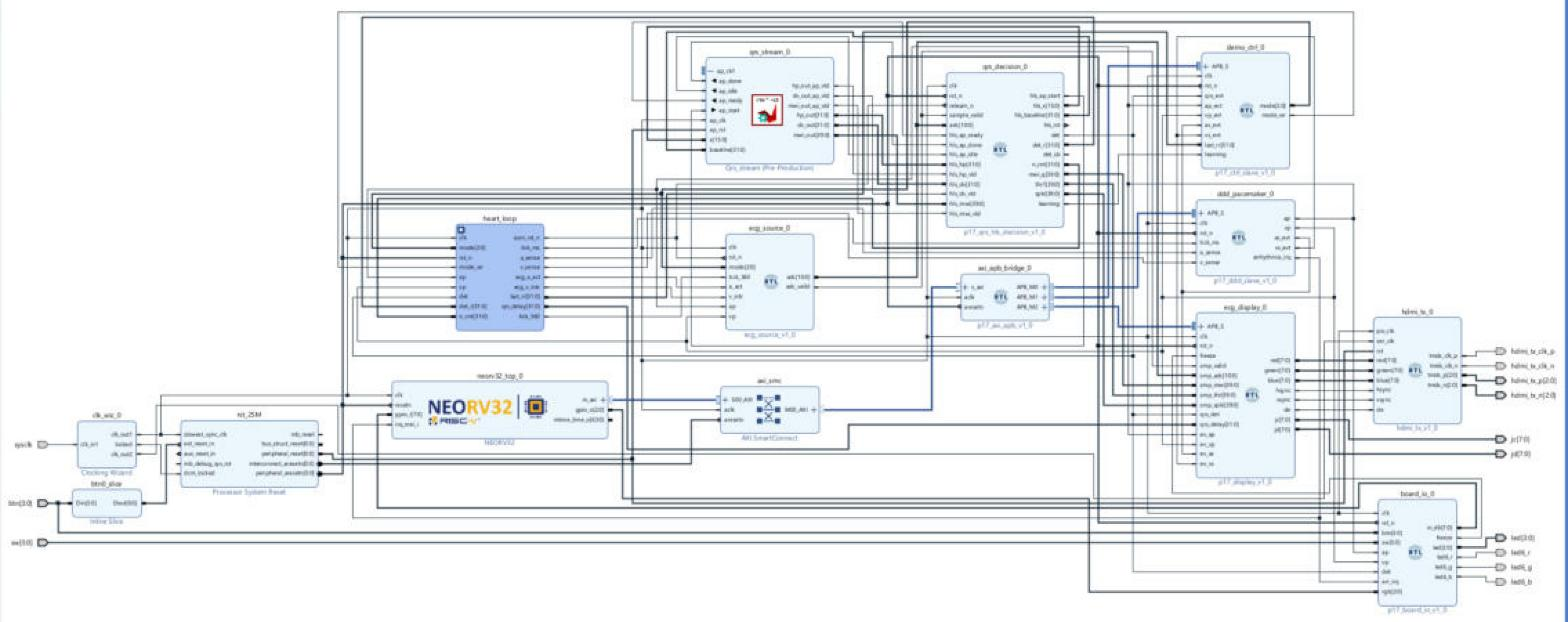
\includegraphics[width=\linewidth]{block_design.jpg}}{\fbox{block\_design.jpg}}
\caption{IP-Integrator block design \texttt{p17\_soc} (NEORV32, SmartConnect, AXI-to-APB bridge, HLS IP, RTL modules).}\label{fig:bd}
\end{figure}

\begin{figure}[H]\centering
\IfFileExists{ila_vivado.jpg}{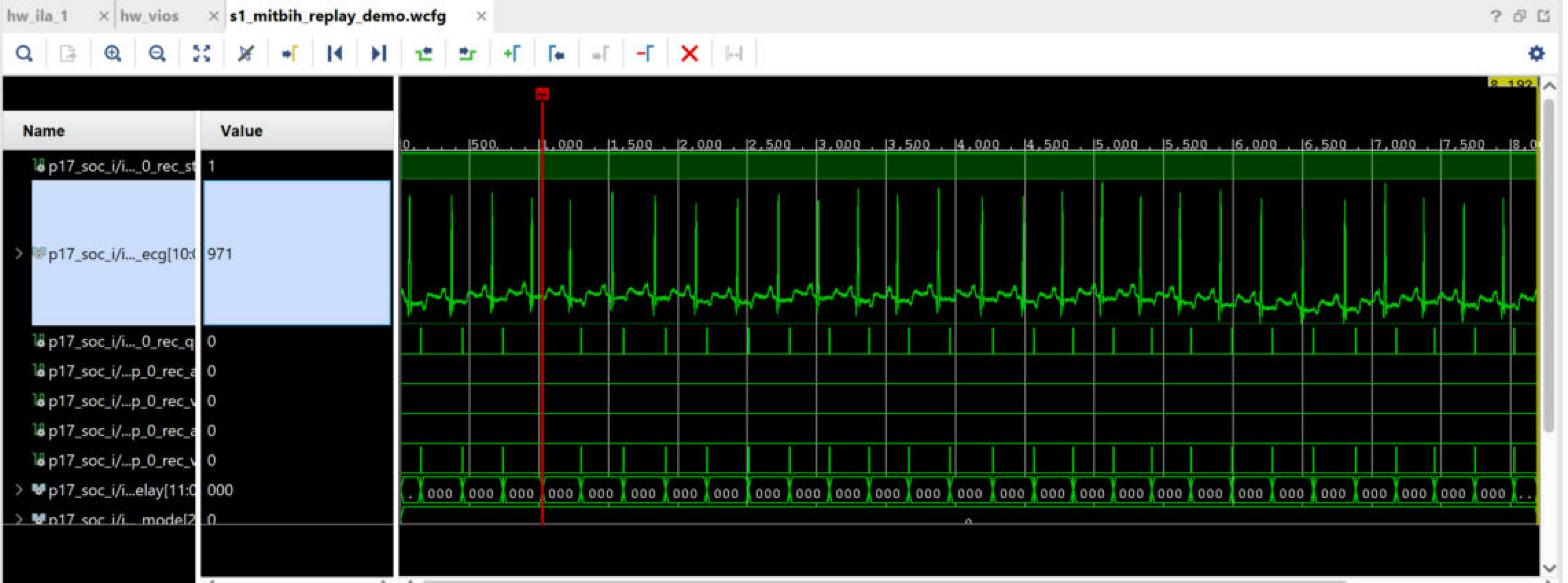
\includegraphics[width=\linewidth]{ila_vivado.jpg}}{\fbox{ila\_vivado.jpg}}
\caption{Vivado Hardware Manager: ILA capture of record 100 on the Zybo, ECG probe shown as an analog waveform with the detected-QRS strobe below.}\label{fig:ilaviv}
\end{figure}

\begin{figure}[H]\centering
\IfFileExists{replay.pdf}{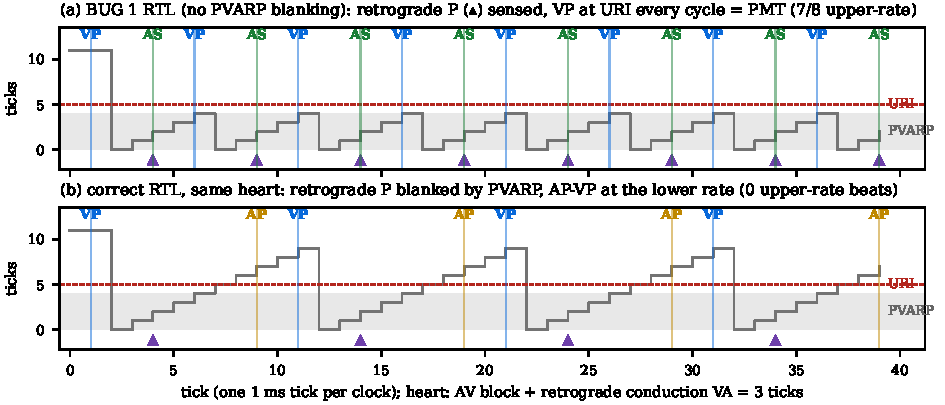
\includegraphics[width=\linewidth]{replay.pdf}}{\fbox{replay.pdf}}
\caption{PMT closed loop on the RTL (xsim): (a) bug-1 mutant, the retrograde P is sensed and VP
lands at URI every cycle; (b) correct RTL, the retrograde P is blanked by PVARP and pacing stays at
the lower rate.}\label{fig:replay}
\end{figure}

\begin{table}[H]\centering\small
\caption{SVA assertions bound to the pacemaker and its APB slave (0 failures in 300{,}000 random + 90{,}000 directed ticks).}\label{tab:svalist}\label{app:sva}
\begin{tabularx}{\linewidth}{@{}lX@{}}
\toprule
Name & Checks that \ldots\\
\midrule
A01--A03 & AP and VP never together; at most one atrial and one ventricular event per tick\\
A04 & every event follows an enabled 1\,ms tick\\
A05, A06 & no V sense inside VRP; no A sense inside PVARP\\
A07, A08 & no VP before URI; no VP before AVI has elapsed\\
A09 & no AP before the atrial escape interval\\
A10 & after each tick $t_v \le \mathrm{LRI}+1$ (saturating timer)\\
A11--A13 & $t_{av}=0$ while waiting for A; a V event restarts the cycle; an A event opens AVI\\
A14 & the upper-rate flag is raised only with a V event\\
A15 & bounded liveness: a V event at least every LRI+1 ticks\\
A16 & APB access phase follows a setup phase\\
A17, A18 & the interrupt latches on the flag and is cleared by write-1-to-clear\\
A19 & no wait states and no error responses\\
C01--C03 & cover: VS and VP at the upper rate; AS followed by VP (all hit)\\
\bottomrule
\end{tabularx}
\end{table}

\begin{table}[H]\centering\small
\caption{Resources per block inside the implemented RTL top (post-route, xc7z010).}\label{tab:perblock}
\begin{tabular}{@{}lccccc@{}}
\toprule
Block & LUT & LUTRAM & FF & BRAM36/18 & DSP\\
\midrule
NEORV32 RV32I (16\,KB IMEM, 8\,KB DMEM) & 1{,}483 & 24 & 1{,}204 & 5 / 4 & 0\\
QRS detector: HLS filter chain & 459 & 162 & 563 & 0 & 3\\
QRS detector: RTL decision & 2{,}730 & 0 & 1{,}704 & 0 & 0\\
DDD pacemaker + APB registers & 236 & 0 & 120 & 0 & 0\\
Heart model & 57 & 0 & 167 & 0 & 0\\
ECG source (MIT-BIH BRAM + templates) & 131 & 0 & 51 & 10 / 0 & 0\\
ECG display (sweep, markers, text) & 736 & 220 & 352 & 2 / 1 & 0\\
Bus bridge / demo control & 77 / 114 & 0 & 70 / 164 & 0 & 0\\
\bottomrule
\end{tabular}
\end{table}


\end{document}
